\documentclass{standalone}
\usepackage{tikz}
\usetikzlibrary{patterns, positioning}


\begin{document}
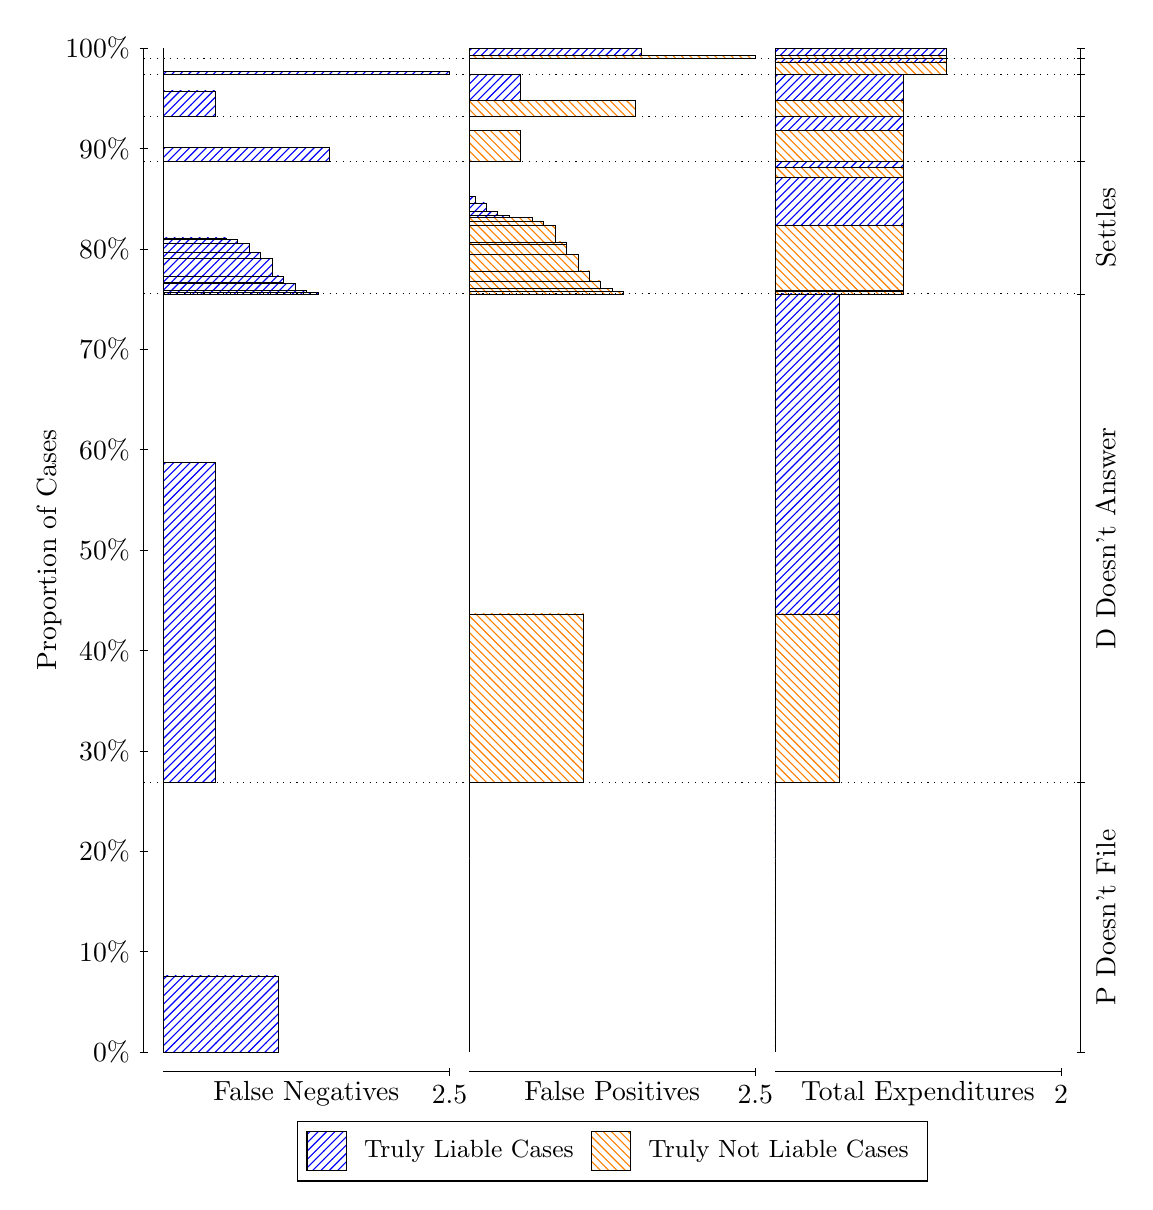
\begin{tikzpicture}
\draw[black, very thin] (1.5,1.75) -- (1.5,14.5);
\node[rotate=90, text=black, anchor=center] at (0.3, 8.125) {Proportion of Cases};
\draw[black, very thin] (1.45,1.75) -- (1.55,1.75);
\node[text=black, anchor=east] at (1.45, 1.75) {0\%};
\draw[black, very thin] (1.45,3.025) -- (1.55,3.025);
\node[text=black, anchor=east] at (1.45, 3.025) {10\%};
\draw[black, very thin] (1.45,4.3) -- (1.55,4.3);
\node[text=black, anchor=east] at (1.45, 4.3) {20\%};
\draw[black, very thin] (1.45,5.575) -- (1.55,5.575);
\node[text=black, anchor=east] at (1.45, 5.575) {30\%};
\draw[black, very thin] (1.45,6.85) -- (1.55,6.85);
\node[text=black, anchor=east] at (1.45, 6.85) {40\%};
\draw[black, very thin] (1.45,8.125) -- (1.55,8.125);
\node[text=black, anchor=east] at (1.45, 8.125) {50\%};
\draw[black, very thin] (1.45,9.4) -- (1.55,9.4);
\node[text=black, anchor=east] at (1.45, 9.4) {60\%};
\draw[black, very thin] (1.45,10.675) -- (1.55,10.675);
\node[text=black, anchor=east] at (1.45, 10.675) {70\%};
\draw[black, very thin] (1.45,11.95) -- (1.55,11.95);
\node[text=black, anchor=east] at (1.45, 11.95) {80\%};
\draw[black, very thin] (1.45,13.225) -- (1.55,13.225);
\node[text=black, anchor=east] at (1.45, 13.225) {90\%};
\draw[black, very thin] (1.45,14.5) -- (1.55,14.5);
\node[text=black, anchor=east] at (1.45, 14.5) {100\%};

\draw[black, very thin] (13.4,1.75) -- (13.4,14.5);
\draw[black, very thin] (13.35,1.75) -- (13.45,1.75);
\node[anchor=west] at (13.35, 1.75) {};
\draw[black, very thin] (13.35,5.1717) -- (13.45,5.1717);
\node[anchor=west] at (13.35, 5.1717) {};
\draw[black, very thin] (13.35,11.379) -- (13.45,11.379);
\node[anchor=west] at (13.35, 11.379) {};
\draw[black, very thin] (13.35,13.063) -- (13.45,13.063);
\node[anchor=west] at (13.35, 13.063) {};
\draw[black, very thin] (13.35,13.631) -- (13.45,13.631);
\node[anchor=west] at (13.35, 13.631) {};
\draw[black, very thin] (13.35,14.162) -- (13.45,14.162);
\node[anchor=west] at (13.35, 14.162) {};
\draw[black, very thin] (13.35,14.366) -- (13.45,14.366);
\node[anchor=west] at (13.35, 14.366) {};
\draw[black, very thin] (13.35,14.5) -- (13.45,14.5);
\node[anchor=west] at (13.35, 14.5) {};

\draw[black, very thin, pattern color=blue, pattern=north east lines] (1.75,1.75) rectangle (3.2033,2.7177);
\draw[black, very thin, pattern color=orange, pattern=north west lines] (1.75,2.7177) rectangle (1.75,5.1717);
\draw[black, very thin, pattern color=blue, pattern=north east lines] (1.75,5.1717) rectangle (2.404,9.2373);
\draw[black, very thin, pattern color=orange, pattern=north west lines] (1.75,9.2373) rectangle (1.75,11.379);
\draw[black, very thin, pattern color=blue, pattern=north east lines] (1.75,11.379) rectangle (3.712,11.399);
\draw[black, very thin, pattern color=blue, pattern=north east lines] (1.75,11.399) rectangle (3.5667,11.421);
\draw[black, very thin, pattern color=blue, pattern=north east lines] (1.75,11.421) rectangle (3.4213,11.511);
\draw[black, very thin, pattern color=blue, pattern=north east lines] (1.75,11.511) rectangle (3.276,11.526);
\draw[black, very thin, pattern color=blue, pattern=north east lines] (1.75,11.526) rectangle (3.276,11.607);
\draw[black, very thin, pattern color=blue, pattern=north east lines] (1.75,11.607) rectangle (3.1307,11.828);
\draw[black, very thin, pattern color=blue, pattern=north east lines] (1.75,11.828) rectangle (2.9853,11.909);
\draw[black, very thin, pattern color=blue, pattern=north east lines] (1.75,11.909) rectangle (2.84,12.015);
\draw[black, very thin, pattern color=blue, pattern=north east lines] (1.75,12.015) rectangle (2.6947,12.069);
\draw[black, very thin, pattern color=blue, pattern=north east lines] (1.75,12.069) rectangle (2.5493,12.088);
\draw[black, very thin, pattern color=orange, pattern=north west lines] (1.75,12.088) rectangle (1.75,13.063);
\draw[black, very thin, pattern color=blue, pattern=north east lines] (1.75,13.063) rectangle (3.8573,13.236);
\draw[black, very thin, pattern color=orange, pattern=north west lines] (1.75,13.236) rectangle (1.75,13.631);
\draw[black, very thin, pattern color=blue, pattern=north east lines] (1.75,13.631) rectangle (2.404,13.956);
\draw[black, very thin, pattern color=orange, pattern=north west lines] (1.75,13.956) rectangle (1.75,14.162);
\draw[black, very thin, pattern color=blue, pattern=north east lines] (1.75,14.162) rectangle (5.3833,14.205);
\draw[black, very thin, pattern color=orange, pattern=north west lines] (1.75,14.205) rectangle (1.75,14.366);
\draw[black, very thin, pattern color=orange, pattern=north west lines] (1.75,14.366) rectangle (1.75,14.409);
\draw[black, very thin, pattern color=blue, pattern=north east lines] (1.75,14.409) rectangle (1.75,14.5);
\draw[black, very thin, pattern color=orange, pattern=north west lines] (5.6333,1.75) rectangle (5.6333,4.204);
\draw[black, very thin, pattern color=blue, pattern=north east lines] (5.6333,4.204) rectangle (5.6333,5.1717);
\draw[black, very thin, pattern color=orange, pattern=north west lines] (5.6333,5.1717) rectangle (7.0867,7.3135);
\draw[black, very thin, pattern color=blue, pattern=north east lines] (5.6333,7.3135) rectangle (5.6333,11.379);
\draw[black, very thin, pattern color=orange, pattern=north west lines] (5.6333,11.379) rectangle (7.5953,11.405);
\draw[black, very thin, pattern color=orange, pattern=north west lines] (5.6333,11.405) rectangle (7.45,11.451);
\draw[black, very thin, pattern color=orange, pattern=north west lines] (5.6333,11.451) rectangle (7.3047,11.543);
\draw[black, very thin, pattern color=orange, pattern=north west lines] (5.6333,11.543) rectangle (7.1593,11.671);
\draw[black, very thin, pattern color=orange, pattern=north west lines] (5.6333,11.671) rectangle (7.014,11.876);
\draw[black, very thin, pattern color=orange, pattern=north west lines] (5.6333,11.876) rectangle (6.8687,12.013);
\draw[black, very thin, pattern color=orange, pattern=north west lines] (5.6333,12.013) rectangle (6.8687,12.038);
\draw[black, very thin, pattern color=orange, pattern=north west lines] (5.6333,12.038) rectangle (6.7233,12.249);
\draw[black, very thin, pattern color=orange, pattern=north west lines] (5.6333,12.249) rectangle (6.578,12.3);
\draw[black, very thin, pattern color=orange, pattern=north west lines] (5.6333,12.3) rectangle (6.4327,12.354);
\draw[black, very thin, pattern color=blue, pattern=north east lines] (5.6333,12.354) rectangle (6.142,12.373);
\draw[black, very thin, pattern color=blue, pattern=north east lines] (5.6333,12.373) rectangle (5.9967,12.426);
\draw[black, very thin, pattern color=blue, pattern=north east lines] (5.6333,12.426) rectangle (5.8513,12.533);
\draw[black, very thin, pattern color=blue, pattern=north east lines] (5.6333,12.533) rectangle (5.706,12.613);
\draw[black, very thin, pattern color=blue, pattern=north east lines] (5.6333,12.613) rectangle (5.6333,13.063);
\draw[black, very thin, pattern color=orange, pattern=north west lines] (5.6333,13.063) rectangle (6.2873,13.457);
\draw[black, very thin, pattern color=blue, pattern=north east lines] (5.6333,13.457) rectangle (5.6333,13.631);
\draw[black, very thin, pattern color=orange, pattern=north west lines] (5.6333,13.631) rectangle (7.7407,13.836);
\draw[black, very thin, pattern color=blue, pattern=north east lines] (5.6333,13.836) rectangle (6.2873,14.162);
\draw[black, very thin, pattern color=orange, pattern=north west lines] (5.6333,14.162) rectangle (5.6333,14.323);
\draw[black, very thin, pattern color=blue, pattern=north east lines] (5.6333,14.323) rectangle (5.6333,14.366);
\draw[black, very thin, pattern color=orange, pattern=north west lines] (5.6333,14.366) rectangle (9.2667,14.409);
\draw[black, very thin, pattern color=blue, pattern=north east lines] (5.6333,14.409) rectangle (7.8133,14.5);
\draw[black, very thin, pattern color=orange, pattern=north west lines] (9.5167,1.75) rectangle (9.5167,4.204);
\draw[black, very thin, pattern color=blue, pattern=north east lines] (9.5167,4.204) rectangle (9.5167,5.1717);
\draw[black, very thin, pattern color=orange, pattern=north west lines] (9.5167,5.1717) rectangle (10.334,7.3135);
\draw[black, very thin, pattern color=blue, pattern=north east lines] (9.5167,7.3135) rectangle (10.334,11.379);
\draw[black, very thin, pattern color=orange, pattern=north west lines] (9.5167,11.379) rectangle (11.152,11.405);
\draw[black, very thin, pattern color=blue, pattern=north east lines] (9.5167,11.405) rectangle (11.152,11.424);
\draw[black, very thin, pattern color=orange, pattern=north west lines] (9.5167,11.424) rectangle (11.152,12.245);
\draw[black, very thin, pattern color=blue, pattern=north east lines] (9.5167,12.245) rectangle (11.152,12.854);
\draw[black, very thin, pattern color=orange, pattern=north west lines] (9.5167,12.854) rectangle (11.152,12.982);
\draw[black, very thin, pattern color=blue, pattern=north east lines] (9.5167,12.982) rectangle (11.152,13.063);
\draw[black, very thin, pattern color=orange, pattern=north west lines] (9.5167,13.063) rectangle (11.152,13.457);
\draw[black, very thin, pattern color=blue, pattern=north east lines] (9.5167,13.457) rectangle (11.152,13.631);
\draw[black, very thin, pattern color=orange, pattern=north west lines] (9.5167,13.631) rectangle (11.152,13.836);
\draw[black, very thin, pattern color=blue, pattern=north east lines] (9.5167,13.836) rectangle (11.152,14.162);
\draw[black, very thin, pattern color=orange, pattern=north west lines] (9.5167,14.162) rectangle (11.697,14.323);
\draw[black, very thin, pattern color=blue, pattern=north east lines] (9.5167,14.323) rectangle (11.697,14.366);
\draw[black, very thin, pattern color=orange, pattern=north west lines] (9.5167,14.366) rectangle (11.697,14.409);
\draw[black, very thin, pattern color=blue, pattern=north east lines] (9.5167,14.409) rectangle (11.697,14.5);
\draw[black, dotted] (1.5,5.1717) -- (13.4,5.1717);
\draw[black, dotted] (1.5,11.379) -- (13.4,11.379);
\draw[black, dotted] (1.5,13.063) -- (13.4,13.063);
\draw[black, dotted] (1.5,13.631) -- (13.4,13.631);
\draw[black, dotted] (1.5,14.162) -- (13.4,14.162);
\draw[black, dotted] (1.5,14.366) -- (13.4,14.366);
\draw[black, very thin] (1.75,1.5) -- (5.3833,1.5);
\node[text=black, anchor=north] at (3.5667, 1.5) {False Negatives};
\draw[black, very thin] (5.3833,1.45) -- (5.3833,1.55);
\node[text=black, anchor=north] at (5.3833, 1.45) {2.5};

\draw[black, very thin] (5.6333,1.5) -- (9.2667,1.5);
\node[text=black, anchor=north] at (7.45, 1.5) {False Positives};
\draw[black, very thin] (9.2667,1.45) -- (9.2667,1.55);
\node[text=black, anchor=north] at (9.2667, 1.45) {2.5};

\draw[black, very thin] (9.5167,1.5) -- (13.15,1.5);
\node[text=black, anchor=north] at (11.333, 1.5) {Total Expenditures};
\draw[black, very thin] (13.15,1.45) -- (13.15,1.55);
\node[text=black, anchor=north] at (13.15, 1.45) {2};

\node[text=black, centered, rotate=90] at (13.72, 3.4608) {P Doesn't File};
\node[text=black, centered, rotate=90] at (13.72, 8.2754) {D Doesn't Answer};
\node[text=black, centered, rotate=90] at (13.72, 12.221) {Settles};





\draw (7.449999999999999,1.5) node[draw=none] (baseCoordinate) {};
\begin{scope}[align=center]
        \matrix[scale=0.5, draw=black, below=0.5cm of baseCoordinate, nodes={draw}, column sep=0.1cm]{
            \node[rectangle, draw, minimum width=0.5cm, minimum height=0.5cm, pattern color=blue, pattern=north east lines] {}; &
            \node[draw=none, font=\small, text=black] (B) {Truly Liable Cases}; &
            \node[rectangle, draw, minimum width=0.5cm, minimum height=0.5cm, pattern color=orange, pattern=north west lines] {}; &
            \node[draw=none, font=\small, text=black] (B) {Truly Not Liable Cases}; \\
            };
\end{scope}

\end{tikzpicture}
\end{document}